\part{Introduction}%
This part of the of the document describes the content of the document and how it should be used, and the changes from version 1.0 of the thesis template.
\chapter{About the template}
\section{What's in this package?}
In this package you will find the following files:
\vspace{1em}
\begin{simplelist}
    \item \textbf{BiblioInfo.tex} - Contains all bibliographic information and information about the defense of the thesis. The author should add this information to the commands defined in this file.
    \item \textbf{Example.tex} - An example to show the typesetting of all the used commands and environments.
    \item \textbf{Instruction.tex} - This file.
    \item \textbf{Introduction.tex} - Tex file for the first chapter.
    \item \textbf{Read.me} - Contains basic instructions for the package.
    \item \textbf{References.bib} - An example of a reference file.
    \item \textbf{Sunset.jpg} - The image in the example.
    \item \textbf{Sunset.eps} - The image in the example.
    \item \textbf{Fonts.pdf} - The image in the instruction.
    \item \textbf{Fonts.eps} - The image in the instruction.    
    \item \textbf{Thesis.blg, Thesis.aux, Thesis.bbl Thesis.log, Thesis.lot, Thesis.out Thesis.toc} - Help files.
    \item \textbf{Thesis.pdf} - The PDF result Thesis.tex.
    \item \textbf{Thesis.ps} - The PostScript result Thesis.tex.
    \item \textbf{Thesis.dvi} - The DVI result Thesis.tex.
    \item \textbf{Thesis.sty} - All the changes to and redefinitions of Book.cls have been collected in this file. It also contains the basic structure of the document along with all new commands and environments used in the template as well as all redefined commands and environments. Since version 3.0 this file defines the commands used in the front matter that create the half-title page, abstractpage, list of papers and dedication.   
    \item \textbf{Thesis.tex} - This is the main \TeX{} file. In this frame all other \TeX{} files are included.
    \item \textbf{UU\_ logo\_ pc\_ sv\_ 42.eps} - The Uppsala University 42 mm black and white logotype in EPS format.
    \item \textbf{UU\_ logo\_ pc\_ sv\_ 42.pdf} - The Uppsala University 42 mm black and white logotype in PDF format.
    \item \textbf{ProblemsAndSolutions.tex} - File containing known problems and suggested solutions.
    \item \textbf{captions.sty} - The used version of caption package. If you miss the latest version of captions use this file.
\end{simplelist}

\section{Instructions}
The template consists of one main file, \emph{Thesis.tex}, and a number of \TeX{} files which are included in the mainfile. The thesis may be split into one or several chapter files which are to be included in the main matter of the Thesis.tex file. Introduction.tex has been included to illustrate this. All the normal commands and environments defined in \LaTeX{} can be used although some of them have been redefined for typographical reasons. In addition to the Thesis.tex the author should edit the BiblioInfo.tex file and use either \textbackslash frontMatterCS or \textbackslash frontmatterMonograph command in the Thesis.tex file to produce the desired result. Finally, Instruction.tex, ProblemsAndSolutions.tex and Example.tex, should be excluded from Thesis.tex after reading them.

\subsection{New environments}
A number of list environments have been added to the template. These are:
\begin{tabbing}
\hspace{4cm}\=\\
enumerate-indent \> Same as enumerate (numbered list) but indented\\
itemize-indent \> Same as itemize (bulleted list) but indented\\
romanlist \> Roman list (Roman numbers)\\
romanlist-indent \> Same as romanlist but indented\\
simplelist \> Simple list (no bullets or numbers)\\
simplelist-indent \> Same as simplelist but indented.
\end{tabbing}

\section{Changes from earlier versions of the \LaTeX{} template}

\subsection{Changes from \LaTeX{} template 4.0.1}
\begin{itemize} 
\item Frontmatter, mainmatter and backmatter commands have all been updated to reflect the recommended style.
\item List of Papers has been added to the pdf bookmarks.
\item Page margins have been redefined.
\item The makeidx package will now produce an entry in table of contents.
\end{itemize} 


\subsection{Changes from \LaTeX{} template 4.0}
\begin{itemize} 
\item All fonts have been redefined to avoid problems using fixed fonts. Math, emphasis and other font commands can be used in the headings without problems.
\item All front matter commands and environments have been moved to the Biblioinfo.tex file for easier editing.
\item The problem with changing the leading of the title on the title page has been solved.
\item The page number on the list of papers page has been removed.
\item The roman list of papers may now be referenced.
\item The booktabs package has been added. It makes it easier to edit nice tables. See the example.
\end{itemize} 


\subsection{Changes from \LaTeX{} template 3.0}
\begin{itemize}
	\item Headings are not forced to break after 3/4 of the complete line width.
	\item FrontMatterMonograph.tex and FrontMatterComrehensiveSummary.tex have been replaced by commands for easier editing of the front matter.
	\item No pages before the first chapter are numbered.
	\item The template now supports both \TeX\(\rightarrow\)DVI\(\rightarrow\)PS generation as well as \TeX\(\rightarrow\)PDF generation.
	\item The template supports Fourier font although Times is still the default font.
	\item Headings are not forced to break after 3/4 of the complete line width.
	\item New environments and commands are moved to Thesis.sty
	\item Penalties for widows and orphans have been increased.
\end{itemize}

\subsection{Changes from \LaTeX{} template 2.2.1}
\begin{itemize}
	\item Headings are ragged right instead of justified.
	\item ISSN and ISBN numbers have changed places.
	\item Hyphenation is allowed in the abstract text but not in the preceding meta data.
\end{itemize}

\subsection{Changes from \LaTeX{} template 2.1}
\begin{itemize}
    \item Headings are forced to break after 3/4 of the complete line width.
    \item \code{\textbackslash emergencystretch} has been increased to avoid overfull \code{hboxes}.
    \item Hyphenation is allowed in the abstract text but not in the preceding meta data.
    \item Hyphenation is not allowed in headings.
    \item The baseline has been corrected for headings.
    \item Heading 1 \ldots Heading 5 have no hanging indents.
    \item Problems and solutions chapter has been added to the documentation.
    \item French spacing is now default.
\end{itemize}


\subsection{Changes from \LaTeX{} template 1.0}
\begin{itemize}
    \item Title page and logos have been removed from Comprehensive summaries. The front matter has been divided into two parts; one for Comprehensive Summaries (FrontMatterComprehensiveSummary.tex) and another for Monographs (FrontMatterMonographs.tex).
    \item List of Papers, the front matter for comprehensive summaries has been simplified.
    \item Hanging indentations for captions have been replaced by non-hanging.
    \item Captions are 10/11p instead of 11/13p.
    \item ActaTable environment has been removed. Font modifications etc. have been included into the common table environment.
    \item Chapters are numbered without chapter marks. Chapter numbers are displayed in the same way as for sections, subsections etc.
    \item Empty pages don't display page numbers.
    \item Spacing above and below equations have been modified to one line of text.
    \item Footnote indentations have been removed.
    \item Changes to the documentclass have been moved to a style-file, Thesis.sty.
    \item The spaces above and below table and figure captions have been modified.
    \item Part command has been redefined to fit monograph authors.
    \item The explanatory part has been extended.
    \item Package \emph{times} has been replaced by \emph{mathptmx} because it's obsolete.
    \item CompehensiveSummary.cls has been replaced by the standard book document class book.cls
    \item Geometry package has been added to set page margins and page size.
\end{itemize}

\section{Important note}
This template may use the pdflatex package to produce the output as a PDF file. The package requires that all images are in JPEG, PNG or PDF  format. EPS files can easily be converted to PDF files using the \emph{ps2pdf} command in the terminal. E.g. ps2pdf imagefile.eps imagefile.pdf. The Linux \emph{convert} command can be used to convert other formats to PDF files. Note that it is not necessary to use the \textit{pdflatex} package and that this version of the template also produces DVI and PostScript files.   

If any of the used packages are missing or out of date in your \LaTeX{} installation, the latest version can be downloaded from http://www.ctan.org/. Packages such as geometry, caption, and many others are typically made
up of two files: a file with the extension .ins and another with the extension .dtx. Run \LaTeX{} on the .ins file.
This will extract a .sty file. Move the .sty file to a place where your distribution can find it. Usually this is in your .../localtexmf/tex/latex subdirectory (Windows or OS/2 users should feel free to change the direction of the slashes). Refresh your distributions file-name database. The command depends on the \LaTeX{} distribution you use: te\TeX{}, fp\TeX{} \code{texhash}; web2c \code{maketexlsr}; Mik\TeX{} \code{initexmf -update-fndb} or use the GUI.
 
\subsection{Fonts}
PDF files created from \LaTeX{} usually don't include embedded fonts. This is due to the fact that the default setting for the distributions in TeX are configured to exclude the 14 basic fonts, for example Times and Helvetica. However, the printers that print dissertations for Uppsala University insist that the fonts are embedded in the PDF so that they can guarantee that the printed version correlates 100\% with the version the author has created. Consequently, the author must change this in his own \TeX{} distribution.

\subsubsection{Mik\TeX{}}
In Mik\TeX{}, this is achieved by changing "psfonts.map" file. This file is in turn governed by a configuration file named "updmap.cfg" found in \textbackslash texmf \textbackslash web2c. 
\begin{enumerate}
	\item Copy updmap.cfg file to \textbackslash localtexmf\textbackslash miktex\textbackslash config.
	\item \raggedright Edit the file and change the setting \code{pdftexDownloadBase14 false} to \code{pdftexDownloadBase14 true} and \code{dvipdfmDownloadBase14 false} to \code{dvipdfmDownloadBase14 true} and finally \code{dvipsDownloadBase35 false} to \code{dvipsDownloadBase35 true}.
	\item Run \code{initexmf --mkmaps} from the command prompt to update psfonts.map.
\end{enumerate}

\vspace{13pt}

\noindent In later Mik\TeX{} versions the procedure is has changed a bit. If the insruction above doesn't work try to
\begin{enumerate}
	\item run \code{initexmf --edit-config-file updmap} from the command prompt.
	\item \raggedright Edit the file and add the text \code{pdftexDownloadBase14 true} and  \code{dvipdfmDownloadBase14 true} and finally \code{dvipsDownloadBase35 true}.
	\item Run \code{initexmf --mkmaps} from the command prompt to update psfonts.map.
\end{enumerate}

\subsubsection{te\TeX{}}
\begin{enumerate}
	\item Run updmap from the command prompt. It gives you information about how fonts ar handled and also what config file is used. For example \code{/usr/local/teTeX/share/texmf.local/web2c/updmap.cfg}.
	\item \raggedright Edit the file and change the setting \code{pdftexDownloadBase14 false} to \code{pdftexDownloadBase14 true} and \code{dvipdfmDownloadBase14 false} to \code{dvipdfmDownloadBase14 true} and finally \code{dvipsDownloadBase35 false} to \code{dvipsDownloadBase35 true}.
		\item Run updmap from the command prompt as super user; \code{sudo updmap} to update psfonts.map.
\end{enumerate}

\subsubsection{How do I know that my fonts are embedded?}
In Acrobat Reader, select File\(\rightarrow\)Document properties\(\rightarrow\)Fonts. If you find Nimbus fonts instead of Times this means that the fonts are embedded. If you use another font i.e. Fourier or Utopia, make sure that there is a \emph{yes} in the embedded column of this dialog.

    \begin{figure}[h!]
        \centering
        \ifpdf
            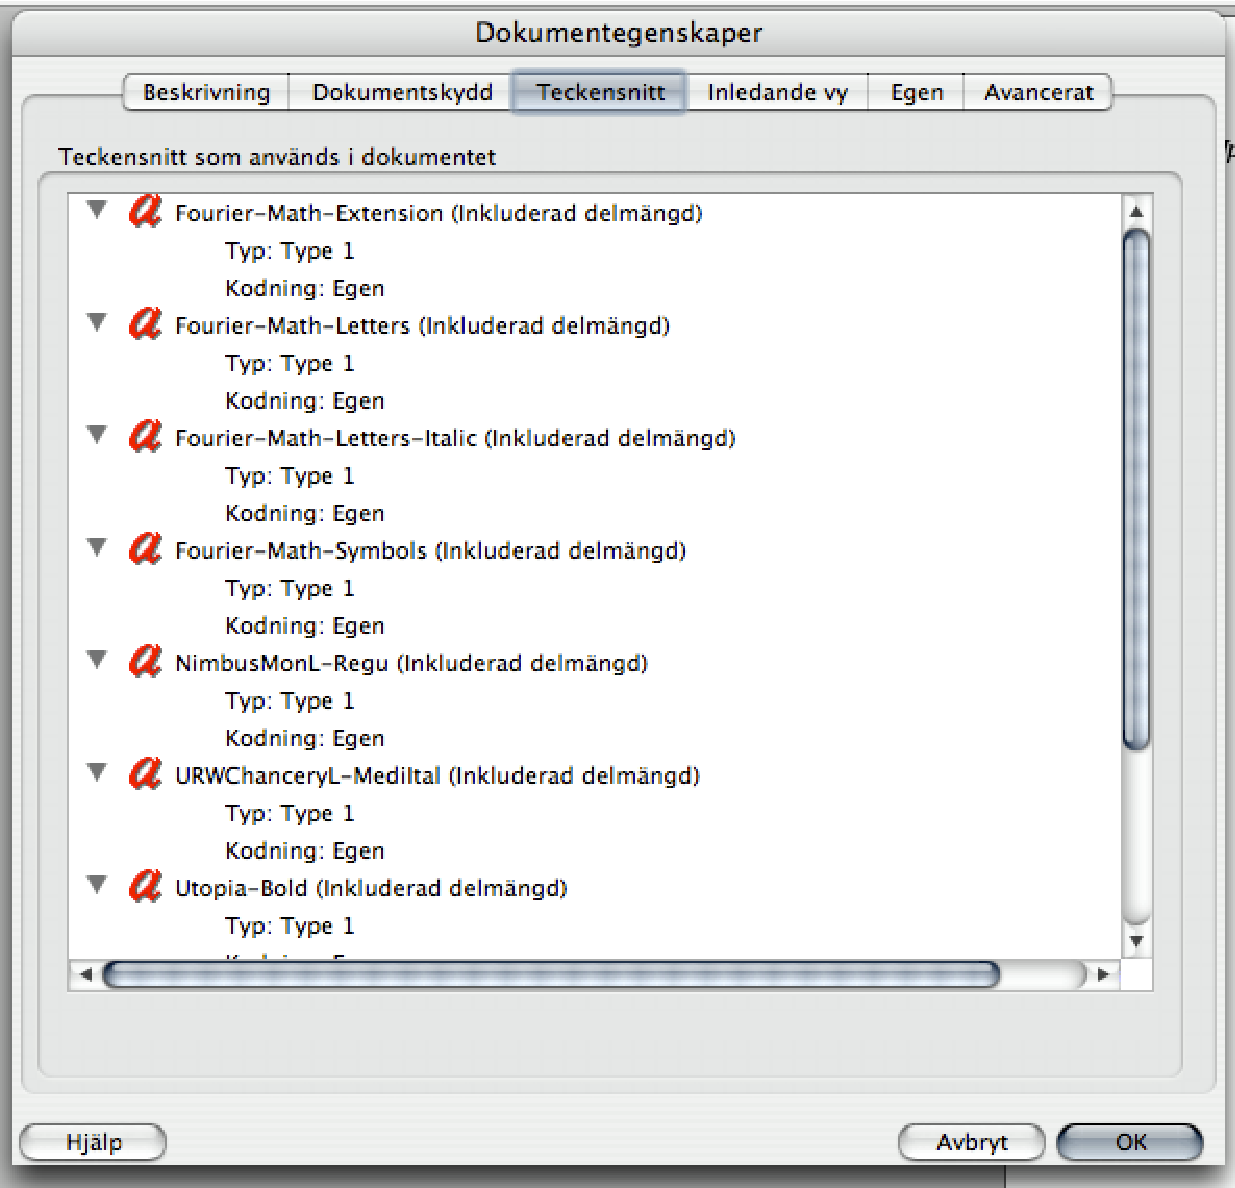
\includegraphics[width=12cm]{Fonts}
        \else
        		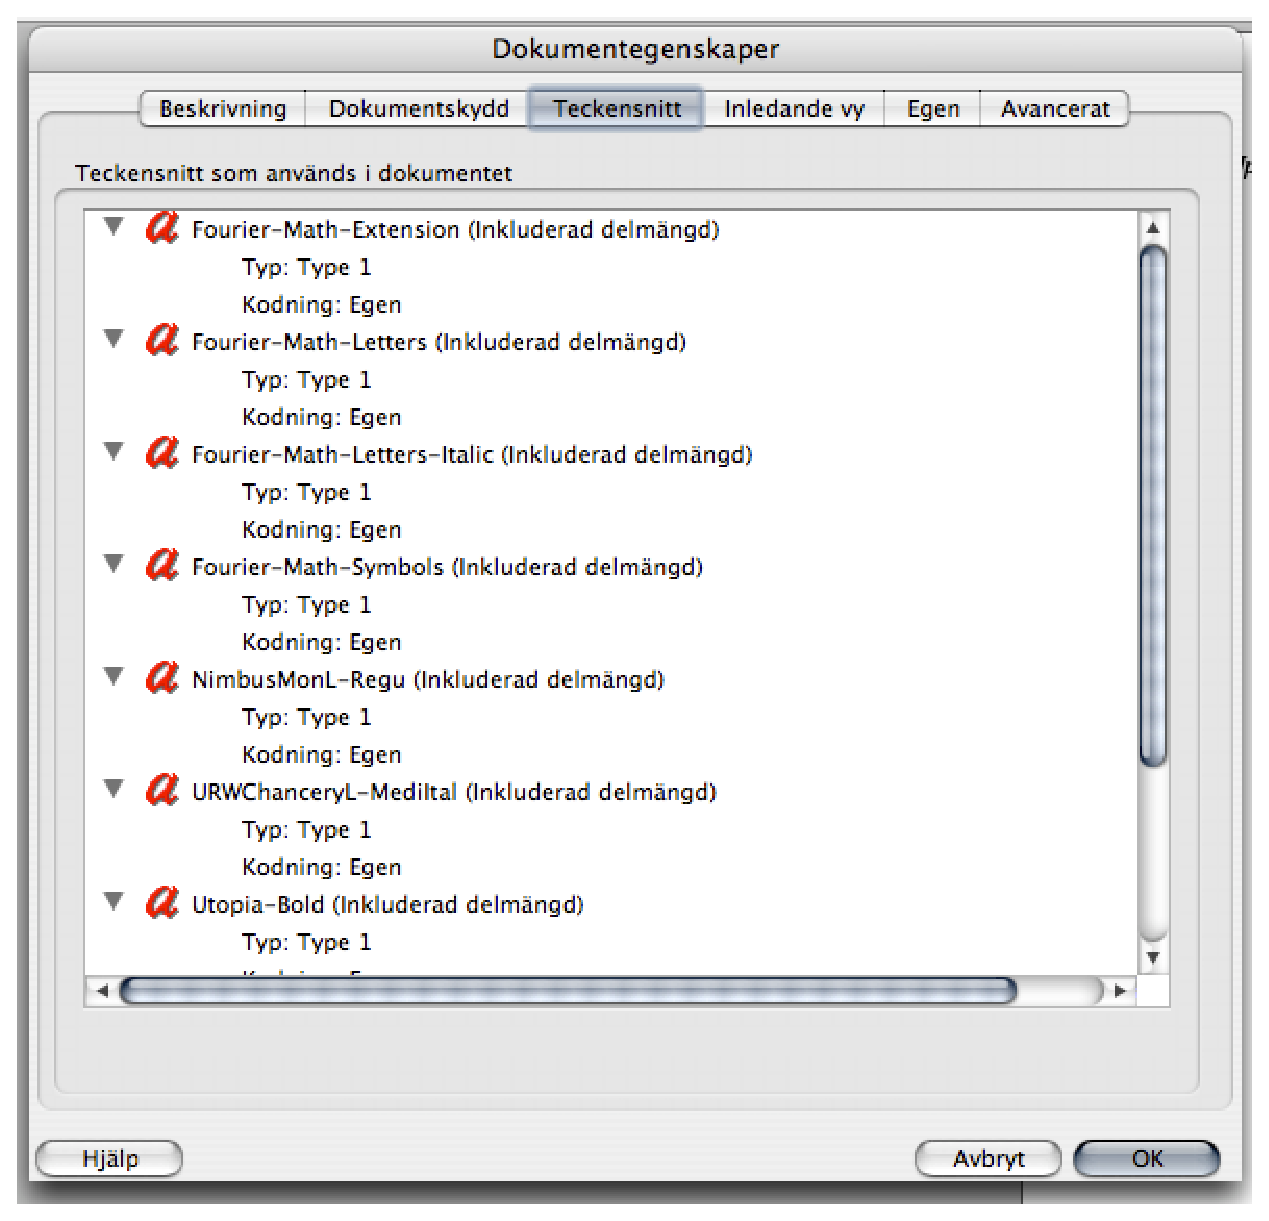
\includegraphics[width=12cm]{Fonts.eps}
		\fi
	\caption{Acrobat document properties and fonts display} 
    \end{figure} 

\vspace{\baselineskip}
\noindent Please send any questions, comments or macro contributions to\\espik@ub.uu.se.

\chapter{About authoring a dissertation\\at Uppsala University}
In order to ensure a uniform layout for, and simplify the making of the dissertations published in the Acta series of Uppsala
University, Publishing and Graphic Services has created a document template for \LaTeXe{}. You find the template "Avhandlingsmall" at \\\href{http://beta.ub.uu.se/en/Service/Publish/For-doctoral-students/Templates-and-PDF-files/}{http://beta.ub.uu.se/en/Service/Publish/For-doctoral-students/Templates-and-PDF-files/}.
\section{Typography}
The template is based on the typography that the Editorial Office at Uppsala University applies to Acta
monographs. The page format is S5 (165 x 242 mm), and the font used throughout is Times with a body text type size of 11 points. The left and right margins are 22,5 mm, and the top and bottom margins are 20 mm.
\section{Outline}
A comprehensive summary should include the following parts in the following order:
\begin{itemize}
    \item Title Page (produced by Publishing and Graphic Services).
    \item Abstract/Imprint page (produced by Publishing and Graphic Services allthough a demo comes with the tempalate).
    \item Dedication page. Optional.
    \item List of Papers.
    \item Table of Contents.
    \item Introduction/Background (the first chapter; the first page to be paginated using Arabic numerals).
    \item Chapter 1 \ldots n.
    \item Summary in Swedish (Mandatory for all Tek-Nat students).
    \item Acknowledgments.
    \item References/Bibliography.
    \item Acta Back Cover (produced by Publishing and Graphic Services).
\end{itemize}
\vspace{1\baselineskip}
A monograph should include the following parts in the following order:

\begin{itemize}
    \item Half-title page.
    \item Title Page.
    \item Abstract/Imprint page (produced by Publishing and Graphic Services allthough a demo comes with the template).
    \item Dedication page. Optional.
    \item Table of Contents.
    \item Introduction/Background (the first chapter; the first page to be paginated using Arabic numerals).
    \item Chapter 1 \ldots n.
    \item Summary in Swedish (Mandatory for all Tek-Nat students).
    \item Acknowledgments.
    \item References/Bibliography.
\end{itemize}
\vspace{1\baselineskip}
\noindent The front matter (the sequence of pages from the half-title page or the title page up to the table of contents) is never paginated. The sequence from Chapter 1 up to References/Bibliography is paginated using Arabic numerals. 
